\chapter{RT-Druid and ERIKA Enterprise tutorial for Altera Nios II}

This small tutorial describes a set of steps needed to design a simple
two CPU multiprocessor application that shows the main features of
\ee\ and \rtd.

This tutorial suppose that the reader is familiar to design of
multiprocessor systems as explained in the Altera document named
{}``Creating Multiprocessor Nios II systems tutorial'' available on
the Altera web site \cite{Altera-multicpu-tutorial}.

The following sections subsumes the Altera tools have been installed
under \file{c:\\altera}. This tutorial has been tested on a Stratix
2s60 evaluation board; This tutorial will work with all Nios II
evaluation boards, because all the specific multiprocessor hardware
involved in the multiprocessor design is a composition of the Altera
Avalon Mutex and of the Altera Avalon PIO peripherals, that are
provided by Altera on all Nios-II supported FPGAs.

Other tutorials are available for download from the Evidence web
site. In particular, we suggest to consider the {\em API Tutorial},
containing a set of demos working on the
\file{standard} and \const{full_featured} single-CPU Altera examples
showing the behavior of the various \ee\ primitives.


\section{The hardware design.}

This Section describes how to create a multicore hardware suitable to
be used with \ee.

There are two options available: use a template design, or
create a design starting from an Altera default example.

\subsection{Importing an already existing hardware design}
Evidence Srl provides an already compiled hardware design that can be
used to test \ee. The hardware design of a four processor demo is
available for download from the Evidence website, under the Nios II
Download section. Please refer to Figure
\ref{fig:tutorial_sopcbuilder_4cpu} for a screenshot of the SOPC
blocks used to create the demo.

To open the demo, you have select ``Restore Archived Project...''
under the Quartus II Project menu. When you select that option, a
dialog box appears. Fill the required informations giving the name of
the QAR file. Please remember that you will have to use the directory of the project inside the OIL file.

The design is basically a modification of the ``standard'' Altera demo
available under
\file{C:\\altera\\81\\nios2eds\\examples\\verilog\\niosII_stratix_2s60_ROHS\\standard}. The
Hardware design is basically a SOPCBuilder block with 4 CPUs, an input
PIO for each processor, and an output PIO plus a mutex connected to
all the CPU data masters. It also includes an SRAM, leds, additional
timers to run FRSH applications, and a bridge to overcome a bug in the
Avalon implementation that appears as a bus lock when more than one
master is present.

\begin{figure}
\begin{center}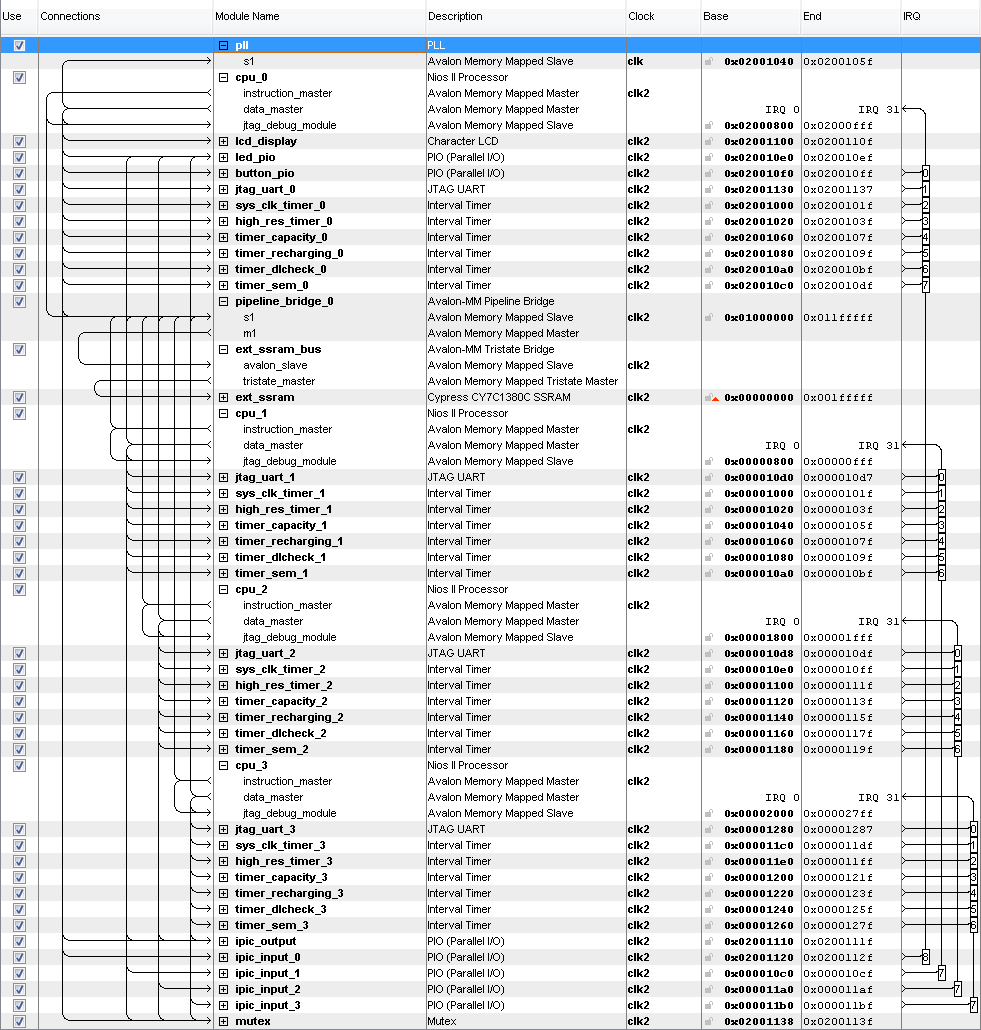
\includegraphics[%
  width=11cm, bb=0 0 981
  1030]{images/frsh_4cpu_sopc_example.png}\end{center}

\caption{\label{fig:tutorial_sopcbuilder_4cpu}The SOPCBuilder blocks created for the 4CPU demo available on the Evidence website.}
\end{figure}

The input and output PIOs are then connected together outside the
SOPCBuilder block to form the InterProcessor Interrupt Controller
(IPIC). Instructions on how to create and connect the various PIO
needed for the Interprocessor interrupt 
are in Section \ref{sec:interprocessor-interrupt}.
can be found inside the \ee\ reference manual.

A SOF file for the example design is already available in the project
directory, so there is no need to recompile the system.

\subsection{Creating an hardware design from scratch}

This subsection describes the steps needed to create an hardware
design suitable for \ee. 

The result will be a dual processor design
that will include all the peripheral needed for a proper
multiprocessor communication; the design will only include standard
Altera SOPCBuilder blocks.

The description is done based on the Altera Stratix II 2s60 Rohs
Evaluation board. Similar results can be obtained using other Altera
evaluation boards.

\begin{enumerate}
\item As the first step, copy the entire directory containing the
  \const{standard} example from Altera in a separate directory called
  \const{evidence_2cpu}. The typical location of the standard example
  is
  \file{c:\\altera\\80\\nios2eds\\examples\\verilog\\boardname\\standard}
  where \const{boardname} is for example
  \const{niosII_cyclone_1c20}. Please create the directory
  \const{evidence_2cpu} at the same level of the \const{standard}
  example directory.



\item Open Quartus II by double clicking on the \file{standard.qpf}
  file inside the \file{evidence_2cpu} directory just created.

\begin{note}
  Some of the new Altera design examples comes with a VHDL/Verilog
  main file instead of the traditional BDF file. We chose to put the
  screenshots of the traditional BDF representation of the project,
  because the graphical representation is easier to understand.
\end{note}



\item Disconnect the pins from the SOPCBuilder Block. Disconnecting the pins
  will help you in the next steps, because the SOPCBuilder block will
  change its size after adding the peripherals described in the
  following paragraphs.


\item Open SOPCBuilder by double clicking on the SOPCBuilder block. A
  window similar to the one showed in Figure
  \ref{fig:tutorial_sopcbuilder_standard} appears.
%
\begin{figure}
\begin{center}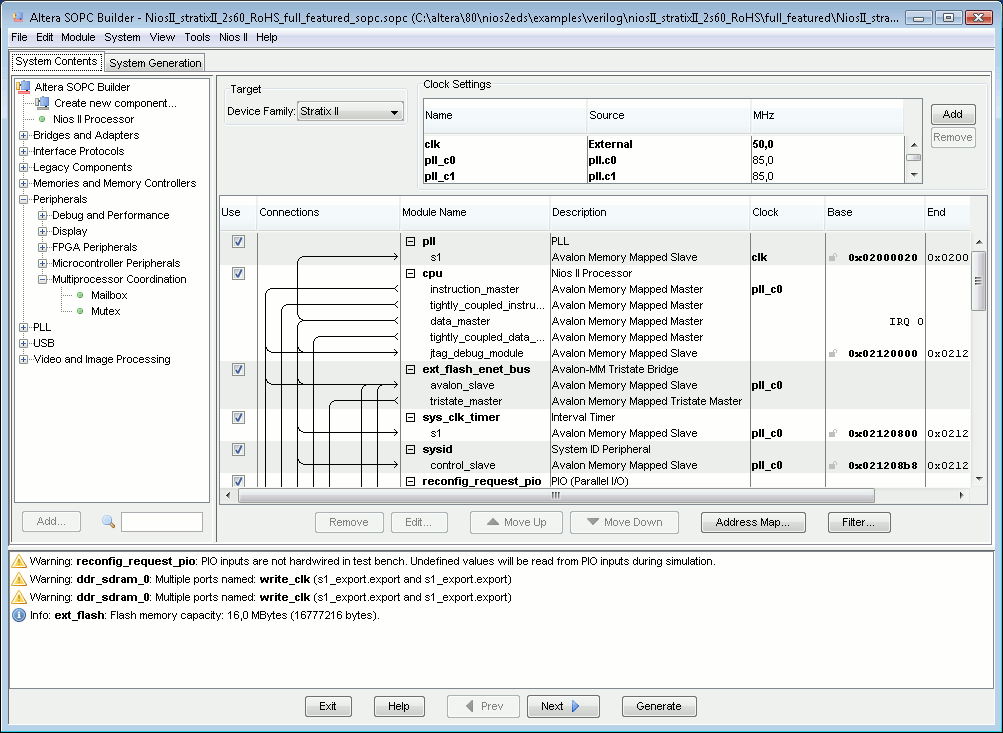
\includegraphics[%
  width=10cm, bb=0 0 1003
  733]{images/tutorial_sopcbuilder.png}\end{center}

\caption{\label{fig:tutorial_sopcbuilder_standard}The SOPCBuilder
windows that appears by opening an Altera project.}
\end{figure}


\item Since multiple instances of some SOPCBuilder components will be
  inserted in the design, change the names of the existing components
  to represent the CPU to which are connected. To rename a component,
  right click on the component name and choose {\em Rename}. First of
  all, rename the CPU from \const{cpu} to \const{cpu_0}.

\item Rename the System Clock Timer from \const{sys_clk_timer}
  to \const{sys_clk_timer_0}.

\item Rename the JTAG UART from \const{jtag_uart} to
  \const{jtag_uart_0}.

\item Rename the High Resolution Timer from \const{high_res_timer} to
  \const{high_res_timer_0}.

\item Add a second CPU named \const{cpu_1}. In the example, we choose
  a Nios II/s, with JTAG debug level 2 (you can leave the other
  options unchanged).

\item Connect both address and data bus of \const{cpu_1} to the
  available memories in the system. Also connect other external buses.

\item Add an Interval Timer component (you can find it under the
  ``Other'' tab of SOPCBuilder) named \const{sys_clk_timer_1}. Set the
  period to 10 ms. This timer is required by the Altera HAL for the
  system clock (see Figure \ref{fig:tutorial_sys_clk_timer}).
%
\begin{figure}
\begin{center}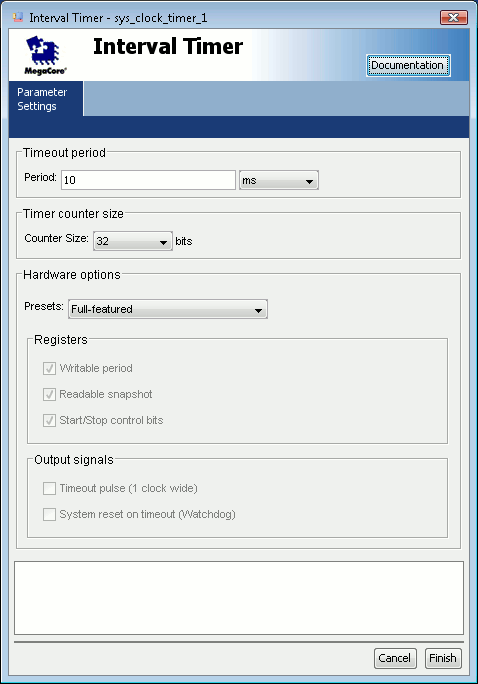
\includegraphics[%
  width=7cm, bb=0 0 478 684]{images/tutorial_sys_clk_timer.png}\end{center}

\caption{\label{fig:tutorial_sys_clk_timer}When creating
\const{sys_clk_timer_1}, use a 10 ms periods.}
\end{figure}

\item Add another Interval Timer named \const{high_res_timer_1}. Leave
  the proposed options unchanged (see Figure
  \ref{fig:tutorial_interval_timer_highres}). This timer is required
  by the Altera HAL for high resolution time measurement.
%
\begin{figure}
\begin{center}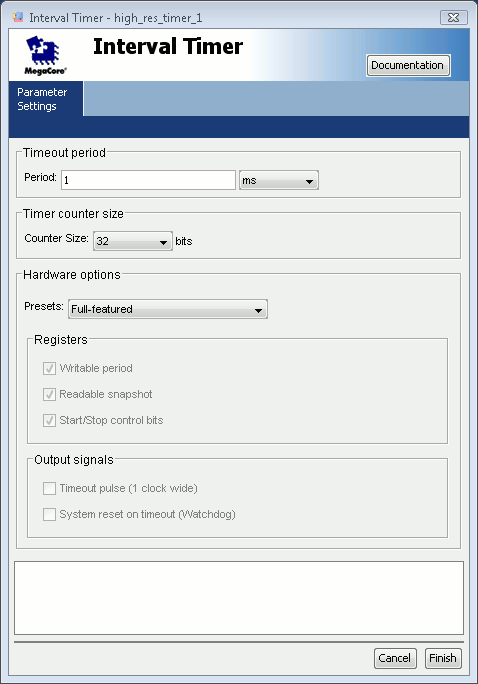
\includegraphics[%
  width=7cm, bb=0 0 478
  684]{images/tutorial_interval_timer_highres.png}\end{center}

\caption{\label{fig:tutorial_interval_timer_highres}When creating
\const{high_res_timer_1}, use a 1 ms periods.}
\end{figure}


\item Add a JTAG Uart (you can find it under the ``Communication'' tab
  of SOPCBuilder) named \const{jtag_uart_1}. Leave the proposed
  options unchanged. The JTAG UART will be used during the software
  example to print some messages on the consoles using printf.

\item Connect the two timers and the JTAG UART only to the data master
  of \const{cpu_1}.

\item At that point, a basic multiprocessor system has been
  created. The resulting system is at this point very similar to the
  one obtained following the Altera Multiprocessor Tutorial
  \cite{Altera-multicpu-tutorial}. The following three paragraphs
  describe the actions to setup the SOPCBuilder components needed to
  implement mutual exclusion between the various CPUs, and to
  implement the interprocessor interrupt controller.

\item Add an Altera Mutex (under the ``Other'' tab of SOPCBuilder)
  named \const{mutex}. Give an ``Initial Value'' equal to \const{0x1},
  and an ``Initial Owner'' equal to \const{0x0}\footnote{The initial
  owner has always value \const{0x0} if you are using Nios II
  6.0. Otherwise, it must be the CPUID of the first CPU (in our case,
  \const{cpu_0}.}. Connect the Altera Mutex peripheral to the data bus
  of both CPUs. Please refer to the \ee\ reference manual for Nios II 
% Section \ref{sec:altera-mutex} and Section \ref{sec:startup-barrier} 
%
  for more information about the usage of the Altera Mutex inside
  hardware designs compatible with \ee.

\item Add an Avalon PIO named \const{ipic_output}. The output PIO
  should have an output bit for each CPU in the system. A screenshot
  of the PIO dialog box can be found in 
  %Section \ref{sec:interprocessor-interrupt}, 
  Figure \ref{fig:IPIC-output}. This
  PIO will be used by the two CPUs to send interprocessor
  interrupts. Connect the PIO to the data master of both CPUs.

\begin{figure}
  \begin{center}
    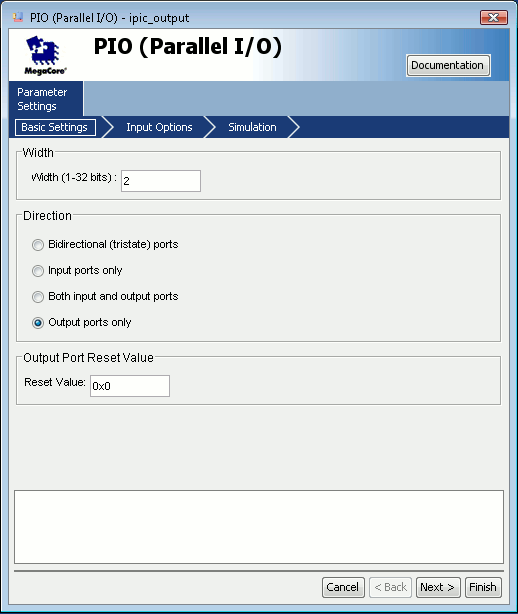
\includegraphics[width=5cm, bb=0 0 518 614]{images/IPIC_PIO_out_dialogbox.png}
    %\pgfimage[width=7cm]{images/IPIC_PIO_out_dialogbox.png}
  \end{center}
  \caption{Output part of the Interprocessor Interrupt. 
    The Figure shows the Avalon PIO output settings.}
  \label{fig:IPIC-output}
\end{figure}


\item Add two Avalon PIOs named \const{ipic_input_0} and
  \const{ipic_input_1}. The PIO must be a 1 bit Input PIO, with
  Synchronous capture on the rising edge, and an Edge IRQ. Screenshots
  of the PIO dialog boxes can be found in 
% Section \ref{sec:interprocessor-interrupt}, 
%
  Figures \ref{fig:IPIC-input-basic}, \ref{fig:IPIC-input-input}, and
  \ref{fig:IPIC-input-simulation}. These PIO will be used by each CPU
  to receive interprocessor interrupts. Connect \const{ipic_input_0}
  to the \const{cpu_0} data bus, and \const{ipic_input_1} to the
  \const{cpu_1} data bus. This is the last component that have to be
  added to SOPCBuilder for this demo. Let's now remove all the errors
  that appears in the bottom of the window, and setup the other tabs
  of SOPCBuilder.


\begin{figure}
  \begin{center}
    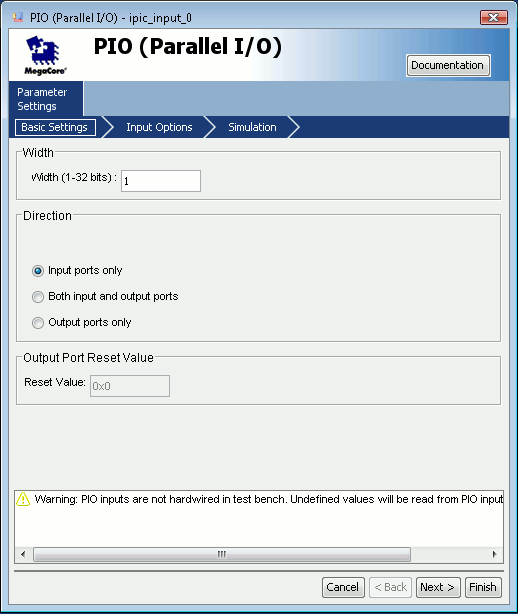
\includegraphics[width=5cm, bb=0 0 518
    614]{images/IPIC_PIO_in_dialogbox_basic.png}
  \end{center}
  \caption{Input part of the Interprocessor 
    Interrupt. The Figure shows the Avalon PIO basic settings.}
  \label{fig:IPIC-input-basic}
\end{figure}

\begin{figure}
  \begin{center}
    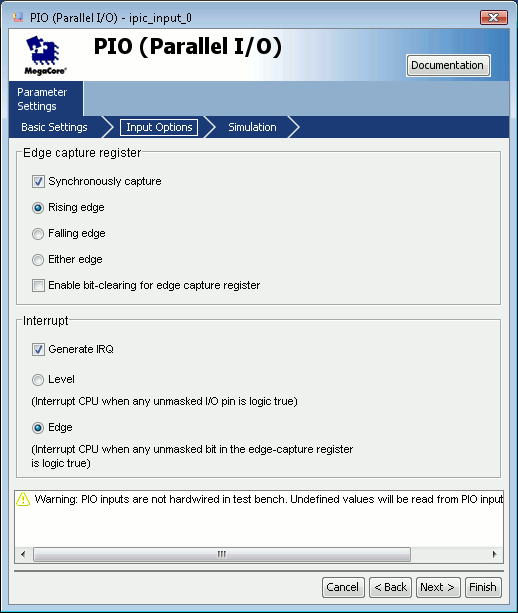
\includegraphics[width=5cm, bb=0 0 518
    613]{images/IPIC_PIO_in_dialogbox_input.png}
    %\pgfimage[width=7cm]{images/IPIC_PIO_in_dialogbox_input.png}
  \end{center}
  \caption{Input part of the Interprocessor Interrupt. 
    The Figure shows the Avalon PIO input settings.}
  \label{fig:IPIC-input-input}
\end{figure}

\begin{figure}
  \begin{center}
    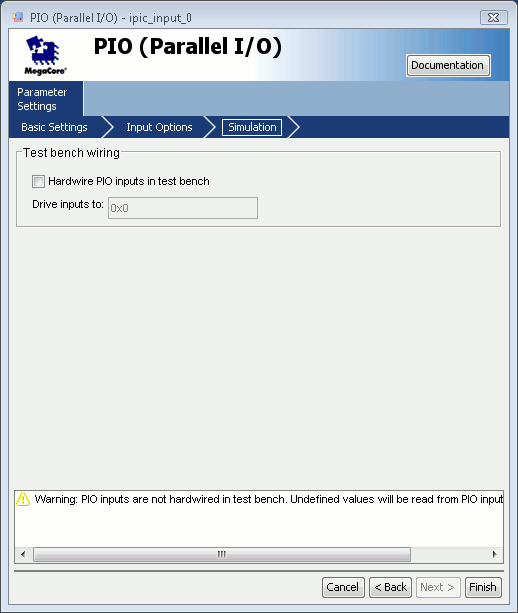
\includegraphics[width=5cm, bb=0 0 518
    613]{images/IPIC_PIO_in_dialogbox_simulation.png}
    %\pgfimage{images/IPIC_PIO_in_dialogbox_simulation.png}
  \end{center}
  \caption{Input part of the Interprocessor Interrupt. 
    The Figure shows the Avalon PIO simulation settings.}
  \label{fig:IPIC-input-simulation}
\end{figure}


\item First of all, IRQ and Base addresses for all the SOPCBuilder
  peripherals have to be set. To do that, execute the commands ``Auto
  Assign Base Addresses'' and ``Auto Assign IRQs'' under the System
  menu.

\item If the design you are developing includes a component connected
  to the external bus, then you have to verify the connections of
  interrupt lines that may be connected to more than one CPU. 
  \begin{warning}
    The interrupt lines of every Altera SOPCBuilder component have to
    be connected to only one CPU!
  \end{warning}
  The \const{standard} example for Stratix 1s40 Evaluation board
  contains an instance of the LAN91c111 SOPCBuilder component. When
  adding the second CPU \const{cpu_1}, SOPCBuilder allows the user to
  set an interrupt line for both CPUs. To solve the problem, you have
  to set the interrupt priority of the \const{cpu_1} connection to
  ``NC'' (Not Connected). A hand-made renumbering of the interrupts
  may also be optionally done.

\item Figure \ref{fig:tutorial_sopcbuilder_final} shows the various
  components and the interrupt connections (the picture was taken
  after removing all the errors in the bottom part of the window as
  discussed in the following paragraphs). The following paragraphs
  discuss the settings of the ``Board Settings'' and the ``Nios II CPU
  Settings'' tabs of SOPCBuilder.
%
\begin{figure}
\begin{center}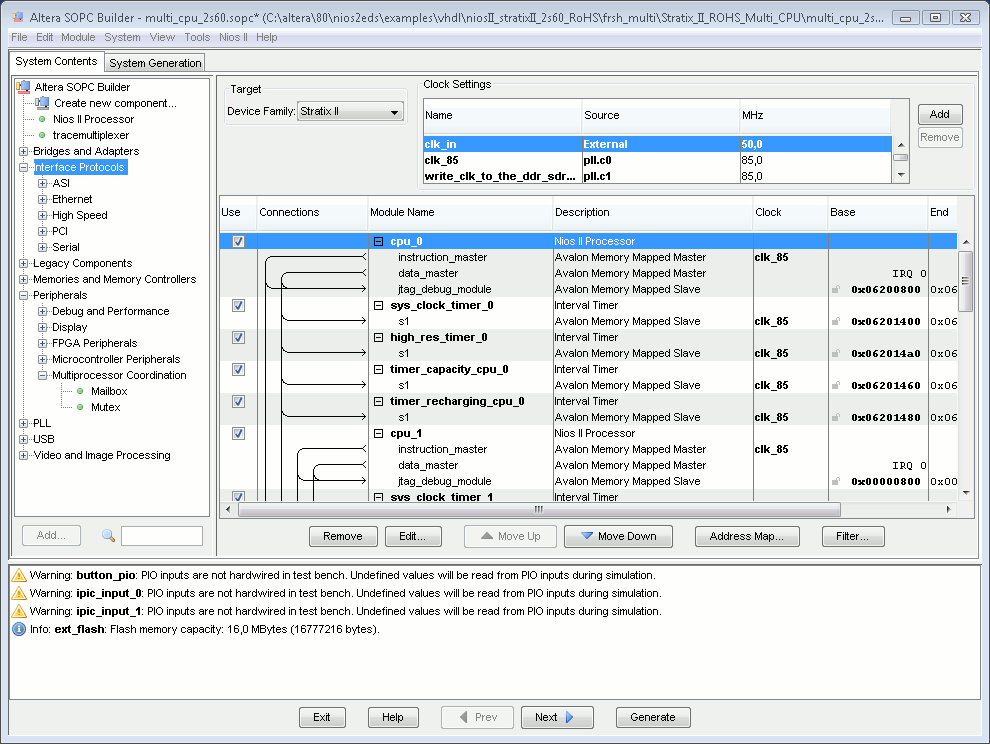
\includegraphics[%
  width=10cm, bb=0 0 1280
  738]{images/tutorial_sopcbuilder_final.png}\end{center}

\caption{\label{fig:tutorial_sopcbuilder_final}The list of SOPCBuilder
components composing this demo.}
\end{figure}

\item Looking at the Board Settings tab, the PIO components used for
  the input and output part of the interprocessor interrupt generate a
  set of unassigned pins. To remove the error, if you are using Nios
  II version 5.0, set the assignment of these pins to ``No
  Assignment''; if you are using Nios II 5.1 or 6.0, as shown in
  Figure \ref{fig:tutorial_boardsettings_after}, set the assignment of
  these pins to ``Assign in Quartus II Project''.
%
%\begin{figure}
%\begin{center}\includegraphics[%
%  width=10cm, bb=0 0 1082 765]{images/tutorial_boardsettings_before.png}\end{center}
%
%\caption{\label{fig:tutorial_boardsettings_before}The Board Settings
%tab before assigning the Interprocessor interrupt pins.}
%\end{figure}
%
\begin{figure}
\begin{center}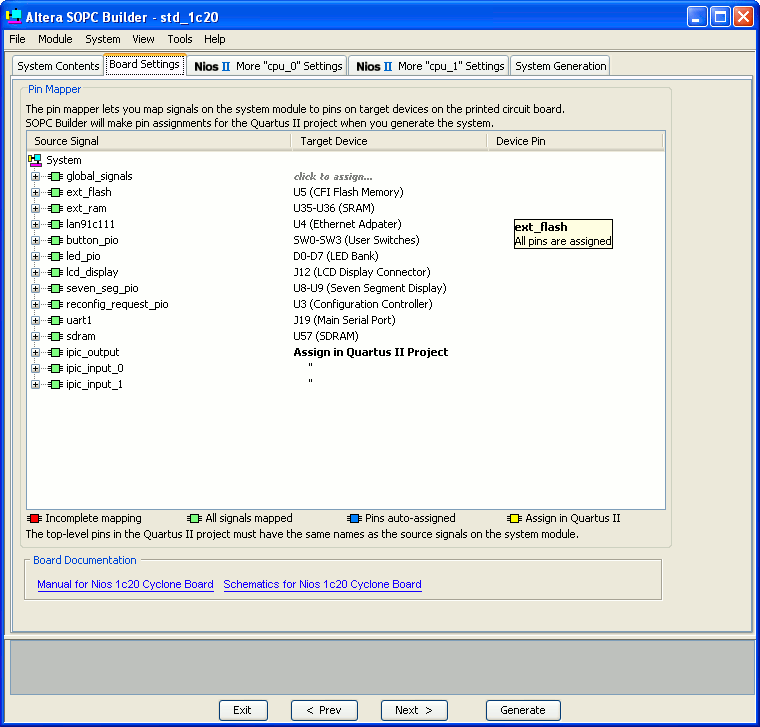
\includegraphics[%
  width=10cm, bb=0 0 760
  727]{images/tutorial_boardsettings_after_1c20.png}\end{center}

\caption{\label{fig:tutorial_boardsettings_after}The Board Settings
tab after assigning the Interprocessor interrupt pins (Nios II Version 5.1 and 6.0).}
\end{figure}

\item As the last thing, set the Reset and Exception address of the
  Nios II CPUs as in Figure \ref{fig:tutorial_cpu0_settings} and
  \ref{fig:tutorial_cpu1_settings}. In this example, the values are
  set considering the following rules:
  \begin{itemize}
    \item The Reset addresses of both CPUs are set to the external
      flash;
    \item The Exception address of both CPUs are set to SDRAM;
    \item The Reset and Exception addresses of \const{cpu_0} are set
      to the start of the respective memories;
    \item The Reset and Exception addresses of \const{cpu_1} are set
      around the middle of the address space of the respective Flash
      and SDRAM memories.
    \item The Reset is always placed at the startup of a flash block
      (see Section \ref{sec:flashing}).
  \end{itemize}
%
\begin{figure}
\begin{center}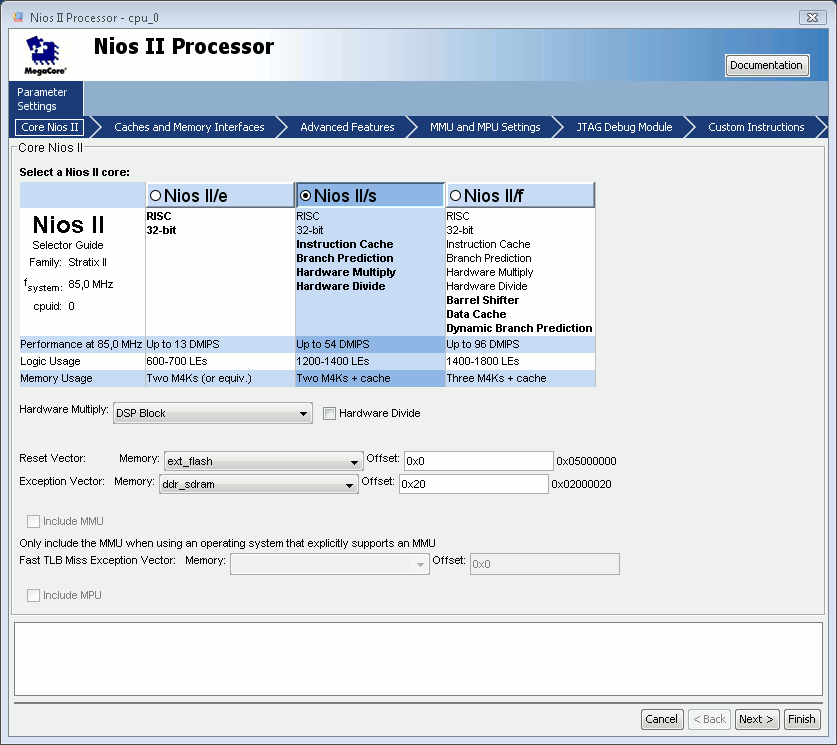
\includegraphics[%
  width=10cm, bb=0 0 837
  745]{images/tutorial_cpu0_settings.png}\end{center}

\caption{\label{fig:tutorial_cpu0_settings}The settings for the \const{cpu_0}.}
\end{figure}
%
\begin{figure}
\begin{center}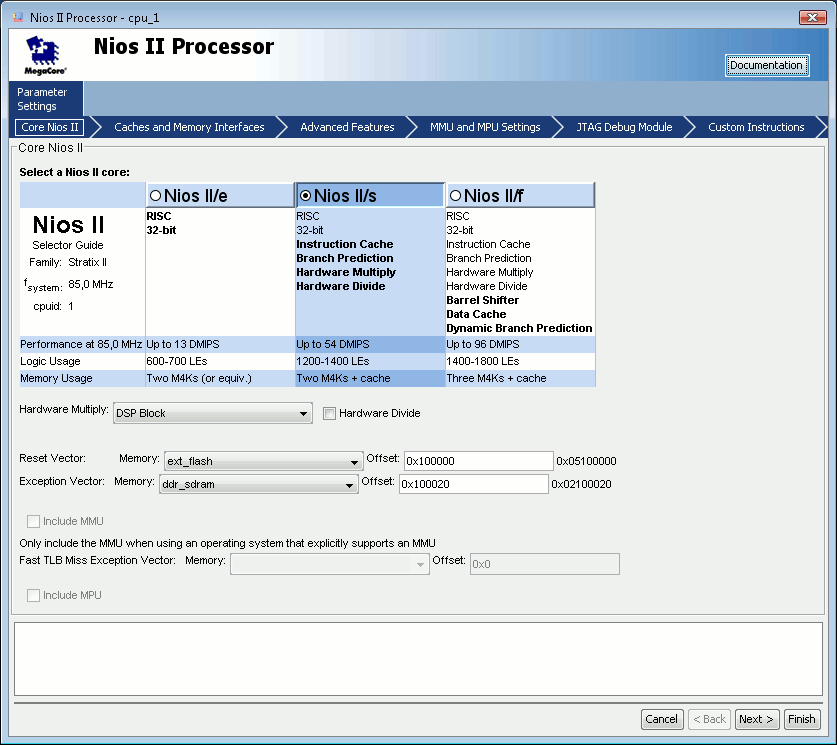
\includegraphics[%
  width=10cm, bb=0 0 837
  745]{images/tutorial_cpu1_settings.png}\end{center}

\caption{\label{fig:tutorial_cpu1_settings}The settings for the \const{cpu_1}.}
\end{figure}

\item Generate the SOPCBuilder Block.

\item As the result of the generation, a .PTF file is created. If you
  are using nios II version 5.0 or 5.1, please check inside the PTF
  File that \const{cpu_0} has CPUID 0, and that \const{cpu_1} has
  CPUID 1. That is important, because as explained in the \ee\
  Reference Manual, %Section \ref{sec:startup-barrier}, the CPUID
  influences the Startup Barrier behavior. The check is not needed if
  you are using nios II 6.0.

\item Go back to Quartus II, and update the symbol. Connect back all
  the various pins of the \const{standard} design, to their respective
  components.

\item Connect the PIO components created for the interprocessor
  interrupt as shown in Figure
  \ref{fig:tutorial_quartus_ipic_pio}. Each pin of the output PIO have
  to be connected to the correspondent CPU. The usage of the named
  pins of Quartus II simplifies the connection. Basically, pin 0 of
  the output PIO have to be connected to the CPU with \const{CPUID} 0
  (typically, \const{cpu_0}); pin 1 of the output PIO have to be
  connected to the CPU with \const{CPUID} 1 (typically,
  \const{cpu_1}), and so on.
%
\begin{figure}
\begin{center}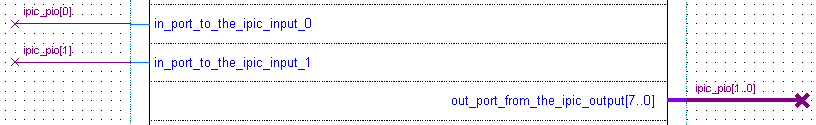
\includegraphics[%
  width=10cm, bb=0 0 816
  125]{images/tutorial_quartus_ipic_pio.png}\end{center}

\caption{\label{fig:tutorial_quartus_ipic_pio}Connecting the output
part of the Interprocessor interrupt to the input part of the
Interprocessor interrupt.}
\end{figure}

\item Finally, you can compile the Quartus II design to produce your
  first design compatible with \ee.
\end{enumerate}



\section{Creating the Altera System Libraries.}

\ee\ applications uses the Altera System Libraries as the base for
linker scripts, boot code and device drivers. This Section shortly
describes which are the main steps to create the System Libraries
needed to be linked to the tutorial application. For more informations
on Altera System Libraries, please refer to official Altera Nios II
documentation.

Open the Nios II IDE from the last SOPCBuilder tab, and select
{}``New'' from the File menu, and then ``Project...''. Choose
{}``System Library'' from the Altera Nios II tab of the New Project
Dialog box. Name the system library \file{evidence_2cpu_cpu0}; the PTF
file of the hardware project should be already selected. Be sure that
\const{cpu_0} is selected.

Repeat the above steps for the second CPU \const{cpu_1}, naming the
second System Library Project as \file{evidence_2cpu_cpu1}, and
selecting \const{cpu_1}.


Build the two system libraries right-clicking on the project name and
choosing ``Build Project''.


\section{The RT-Druid Project}

Open the Nios II IDE from SOPCBuilder, and select ``New Project...''
from the File menu. Choose ``RT-Druid Nios Project'' from the Evidence
tab of the New Project Dialog box. A dialog box appears.  Choose the 2 CPu demo, as shown in Figure \ref{multicore_template}. Name the
project \file{evidence_2cpu} and press the Finish button.

%
\begin{figure}
\begin{center}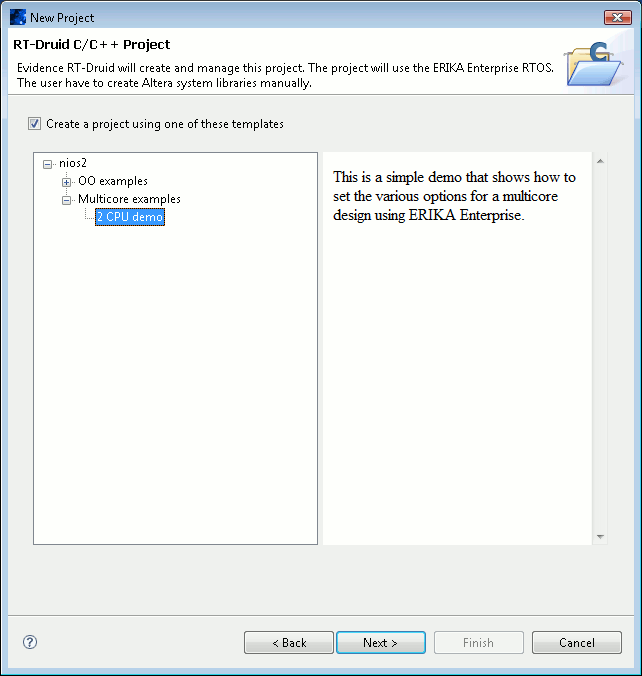
\includegraphics[%
  width=8cm, bb=0 0 642 676]{images/multicore_template.png}\end{center}


\caption{\label{fig:multicore_template}Selecting the Multicore template. }
\end{figure}




\section{Updating the OIL File}

This Section asks you to change the OIL file inserting the locations
of the system libraries you just created. You need to do that only if
the system library names and locations you chose are not the ones
specified in this tutorial. You can go directly to the next Section if
you chose the file names specified early in this tutorial.

Inside the OIL file, look for the \const{CPU_DATA} sections located at
the top of the OIL description inside the \const{OS} section. There is
a \const{CPU_DATA} section for each CPU in the system. Each section
has two settings, called \const{SYSTEM_LIBRARY_NAME} and
\const{SYSTEM_LIBRARY_PATH}. You need to change them with the real
names of the system libraries. When specifying the pathnames, please
use the slash (\file{/}) character and not the backslash (\file{\\})
character. These two settings will be used in the makefiles that are
automatically generated by \rtd\footnote{If unsure on the value to
put in these variables, you can do in one of the following two ways:
\begin{itemize}
\item create a normal Altera project for one of the CPUs (for example,
  a Hello World application), linking it to the System library you
  want to use on the particular CPU. Then, compile the Altera
  application, and look at the file \file{Debug/makefile} inside the
  Altera project.  The value of the \const{SYSTEM_NAME} variable is
  the value that have to be put in the OIL tag
  \const{SYSTEM_LIBRARY_NAME}; the value of the variable
  \const{SYSTEM_DIR} is the value of the OIL tag
  \const{SYSTEM_LIBRARY_DIR}.
\item a faster way to fill the \const{SYSTEM_LIBRARY_PATH} variable is
  to open the properties of the Altera System Libraries, and then look
  at the ``Location'' value inside the info tab. Note that you have to
  substitute \file{\\} with \file{/}.
\end{itemize}
}.


\section{Compiling the application}
Right click on the project name, and select ``Build
Project''.  The demo application will be compiled, and two ELF
binaries will be produced.




\section{Running the application}

First of all, check if the ``Allow multiple active run/debug
sessions'' option has been enabled in the Nios II preferences (see
Figure \ref{fig:tutorial-niospreferences}).

%
\begin{figure}
\begin{center}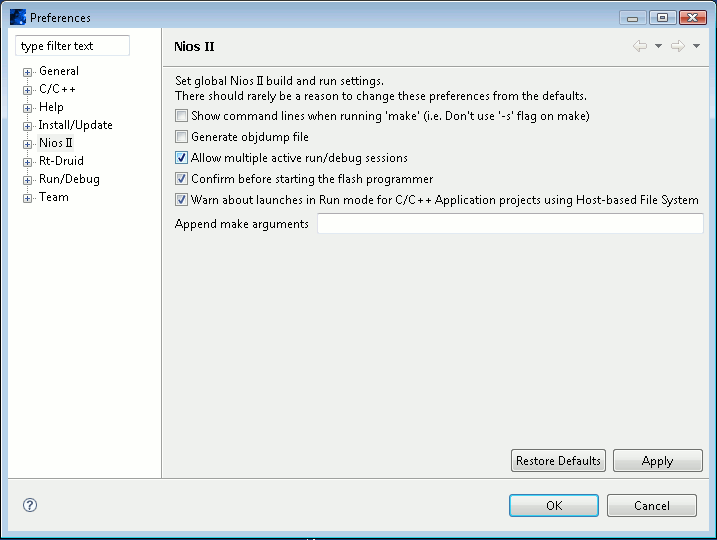
\includegraphics[%
  width=8cm, bb=0 0 717
  540]{images/Nios2_preferences.png}\end{center}


\caption{\label{fig:tutorial-niospreferences}Enabling multiprocessor
debugging in the Nios II preferences.}
\end{figure}


Then, click on the {}``Run...'' option in the toolbar. A dialog box
appears allowing the specification of the Debug configurations.
Create a Nios II Hardware configuration for each CPU in the system.
For each configuration:

\begin{itemize}
\item in the Target Hardware frame, select the project PTF file, and
  the right CPU in the system;
\item in the Nios II ELF Executable text box, please select the Nios
  II ELF executable for the selected CPU;
\item do not forget to click on the ``Target Connection'' tab and
  check that the correct JTAG UART has been automatically selected.
\end{itemize}

Finally, create a Nios II Multiprocessor collection grouping all the
Hardware configurations just created.

You are now ready to start the multiprocessor application. Every time
you want to run a Multiprocessor application, you have to:

\begin{itemize}
\item open the Quartus II Programmer under the Tools menu, and program
  the SOF file you find in the Hardware project directory. 
  \begin{warning}
    You need to reprogram the FPGA every time you start a debug
    session, because the Altera Mutex peripheral is not reset to its
    initial value upon a Debug Stop.
  \end{warning}
\item choose the Multiprocessor Collection Debug configuration when
  pressing the ``Run...'' button.
\end{itemize}
When running the application, the following behavior happens:

\begin{itemize}
\item Both CPUs start in Debug mode (or Run mode if you selected that).
\item Both CPUs print a message like the following one:
\begin{lstlisting}
Hello from CPU 0!

Press a button to activate the tasks...
\end{lstlisting}

\item The two CPUs synchronize at the startup barrier inside the
  \fn{StartOS()} primitive inside \fn{main()}.
\item When both CPUs enters the \fn{StartOS()} primitive, the
  synchronization barrier is passed, and the \fn{StartOS()} primitive
  returns.

\item Press one of the buttons on the evaluation board.  The press of
  the button provoke the activation of three threads. Each thread
  prints a message on the console of the CPU where it is allocated to.
  In the configuration shipped with \ee\, task 0 and 1 are
  allocated on CPU 0, whereas task 2 is allocated to CPU 1.
\end{itemize}

\section{Partitioning the software}

\rtd\ and \ee\ allow an easy partitioning of the application
software. Changing the partitioning of the tasks into the CPUs is very
simple: you just need to change the \const{CPU_ID} parameter in the
task section of the OIL file.

For example, you can put all the three tasks to CPU 0, or the tasks to
CPU 1, or choose an intermediate partitioning. In all these cases,
multiprocessor resource handling and task activations will be hided by
\ee, without changing the application software.  Please note
that a different partitioning scheme does not require a change in the
application source code, but only in the OIL configuration file.

To test a different partitioning, just change the OIL File, recompile
and rerun the demo.




\section{Flashing the demo on the evaluation board}
\label{sec:flashing}

The last phase in the development of a multiprocessor design using
Nios II is typically the flashing of the demo on the flash device that
is usually present in the development (or production) board.

To do that, open the Flash Programmer (under the Tools menu of the
Nios II IDE), and create one configuration for each CPU. Each
configuration for each CPU should specify the PTF file of the
multiprocessor design, selecting the appropriate cpu and ELF
file. Moreover, the first CPU should also include the flashing of the
SOF file. Figure \ref{fig:tutorial-flash-programmer-cpu0} and
\ref{fig:tutorial-flash-programmer-cpu0} show a typical configuration
of the flash programmer for the CPU 0 and 1 of the 2 CPU demo showed
in this tutorial. As you can see, the SOF file is only included in the
flash configuration of CPU 0.

Please note that this way of flashing the data to the evaluation board
flash memory depends on the reset addresses used for the CPUs in
SOPCBuilder. The reset addresses, in particular, have been chosen to
have non-overlapping flash regions for each CPU.

%
\begin{figure}
\begin{center}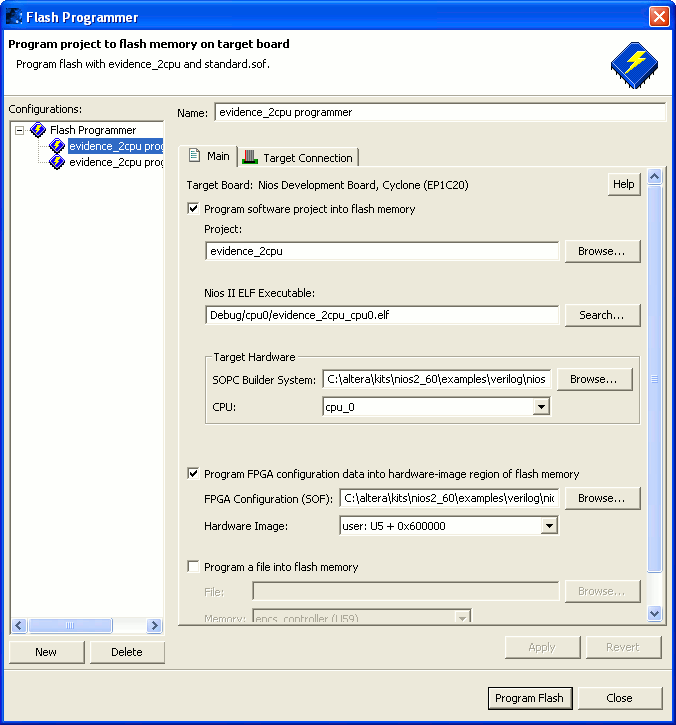
\includegraphics[%
  width=10cm, bb=0 0 676
  725]{images/tutorial_flash_programmer_cpu0_1c20.png}\end{center}


\caption{\label{fig:tutorial-flash-programmer-cpu0}The Flash
Programmer configuration for CPU 0.}
\end{figure}

%
\begin{figure}
\begin{center}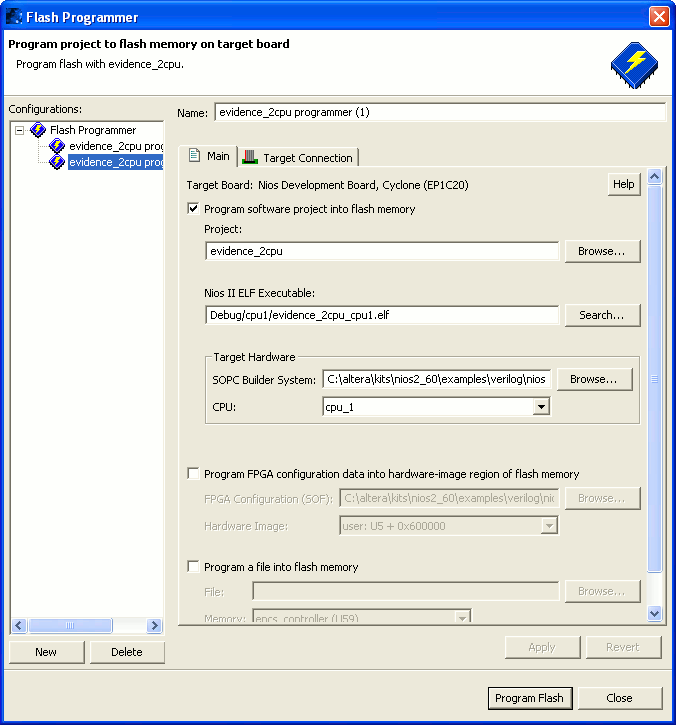
\includegraphics[%
  width=10cm, bb=0 0 676
  725]{images/tutorial_flash_programmer_cpu1_1c20.png}\end{center}


\caption{\label{fig:tutorial-flash-programmer-cpu1}The Flash
Programmer configuration for CPU 1.}
\end{figure}

\begin{warning}
Some care have to be used when defining the addresses that will be
used in the flash.

Flash memories, in fact, are divided in blocks. The flash memory
programming model says that flash devices can be written and erased
with a granularity of a block.

When writing the software for the Nios II platform, each CPU produces
a separate ELF file, that is typically programmed separately using the
Altera Flash Programmer tool.

It is important that each flash block contains data coming from a
single ELF image. To do that, reset addresses of each CPU in
SOPCBuilder have to be set preferably to the starting address of a
flash block. Figure \ref{fig:tutorial-flash-error} gives an example of
the erroneous situation.

As an alternative, the various flash images from each CPU have to be
packed together in a single flash programming file.
\end{warning}

%
\begin{figure}
\includegraphics[%
  width=1\columnwidth]{images/tutorial_flash_error.eps}
\caption{\label{fig:tutorial-flash-error}This Figure shows a typical
flash memory layout highlighting the error situation that appears when
a flash block contains data from two CPUs.}
\end{figure}

\begin{warning}
If you are using onchip memories, after compiling the software to be
flashed, remember to run again the Quartus II Assembler to include the
generated hex files for these memories inside the SOF file.
\end{warning}

After that, run the flashing procedure from the Altera Flash
Programmer. The following lines show a typical output of the flash
programmer.

For CPU 0:

\begin{lstlisting}[basicstyle=\scriptsize\ttfamily]
#! /bin/sh
#
# This file was automatically generated by the Nios II IDE Flash Programmer.
#
# It will be overwritten when the flash programmer options change.
#

cd c:/altera/kits/nios2/bin/eclipse/workspace3/demo_2cpu/Debug/cpu0

# Creating .flash file for the FPGA configuration
$SOPC_KIT_NIOS2/bin/sof2flash --flash=U5 --offset=0x400000 
  --input=$SOPC_KIT_NIOS2/examples/verilog/niosII_stratix_1s40/evidence_2cpu/standard.sof 
  --output=standard.flash
Info: *******************************************************************
Info: Running Quartus II Convert_programming_file
Info: Command: quartus_cpf --no_banner --convert 
  C:/altera/kits/nios2/examples/verilog/niosII_stratix_1s40/evidence_2cpu/standard.sof 
  standard.rbf
Info: Quartus II Convert_programming_file was successful. 0 errors, 0 warnings
    Info: Processing ended: Thu Oct 27 09:36:08 2005
    Info: Elapsed time: 00:00:02

# Programming flash with the FPGA configuration
$SOPC_KIT_NIOS2/bin/nios2-flash-programmer --input=standard.flash 
  --sof=$SOPC_KIT_NIOS2/components/altera_nios_dev_board_stratix_1s40/system/
    altera_nios_dev_board_stratix_1s40.sof 
  --base=0x00800000
27-ott-2005 9.36.13 - (INFO) nios2-flash-programmer: 
  Launching Quartus Programmer to download:
     C:/altera/kits/nios2/components/altera_nios_dev_board_stratix_1s40/system/
       altera_nios_dev_board_stratix_1s40.sof
Pre-Reading 1520KBytes of data from U5:
    |----.----+----.----|
    ********************* (12.312 sec).
Erasing 24 Sectors:
    |----.----+----.----|
    ********************* (15.61 sec).
Writing 1536KBytes :
    |----.----+----.----|
    ********************* (48.0 sec).
Verifying 1536KBytes of data:
    |----.----+----.----|
    ********************* (11.593 sec).
27-ott-2005 9.37.49 - (INFO) nios2-flash-programmer: 
  Success. Verified 1536Kbytes written to U5.
27-ott-2005 9.37.49 - (INFO) nios2-flash-programmer: 
  Flash programming complete

# Creating .flash file for the project
$SOPC_KIT_NIOS2/bin/elf2flash --flash=U5 --base=0x00000000 --end=0x7fffff 
  --reset=0x0 --input=demo_2cpu_cpu0.elf --output=ext_flash.flash 
  --boot=$SOPC_KIT_NIOS2/components/altera_nios2/boot_loader_cfi.srec

# Programming flash with the project
$SOPC_KIT_NIOS2/bin/nios2-flash-programmer --input=ext_flash.flash 
  --sof=__NO_SOF_PLEASE__ --base=0x00800000
27-ott-2005 9.37.50 - (INFO) nios2-flash-programmer: SOF-download skipped.
Pre-Reading 72KBytes of data from U5:
    |----.----+----.----|
    ********************* (1.125 sec).
Erasing 2 Sectors:
    |----.----+----.----|
    ********************* (1.438 sec).
Writing 128KBytes :
    |----.----+----.----|
    ********************* (3.609 sec).
Verifying 128KBytes of data:
    |----.----+----.----|
    ********************* (1.312 sec).
27-ott-2005 9.38.00 - (INFO) nios2-flash-programmer: 
  Success. Verified 128Kbytes written to U5.
27-ott-2005 9.38.00 - (INFO) nios2-flash-programmer: 
  Flash programming complete
\end{lstlisting}




For CPU 1:


\begin{lstlisting}[basicstyle=\scriptsize\ttfamily]
#! /bin/sh
#
# This file was automatically generated by the Nios II IDE Flash Programmer.
#
# It will be overwritten when the flash programmer options change.
#

cd c:/altera/kits/nios2/bin/eclipse/workspace3/demo_2cpu/Debug/cpu1

# Creating .flash file for the project
$SOPC_KIT_NIOS2/bin/elf2flash --flash=U5 --base=0x00000000 --end=0x7fffff --reset=0x100000 
  --input=demo_2cpu_cpu1.elf --output=ext_flash.flash 
  --boot=$SOPC_KIT_NIOS2/components/altera_nios2/boot_loader_cfi.srec

# Programming flash with the project
$SOPC_KIT_NIOS2/bin/nios2-flash-programmer --input=ext_flash.flash 
  --sof=$SOPC_KIT_NIOS2/components/altera_nios_dev_board_stratix_1s40/system/
    altera_nios_dev_board_stratix_1s40.sof --base=0x00800000
27-ott-2005 9.39.54 - (INFO) nios2-flash-programmer: 
  Launching Quartus Programmer to download:
     C:/altera/kits/nios2/components/altera_nios_dev_board_stratix_1s40/system/
       altera_nios_dev_board_stratix_1s40.sof
Pre-Reading 66KBytes of data from U5:
    |----.----+----.----|
    ********************* (1.125 sec).
Erasing 2 Sectors:
    |----.----+----.----|
    ********************* (1.86 sec).
Writing 128KBytes :
    |----.----+----.----|
    ********************* (3.531 sec).
Verifying 128KBytes of data:
    |----.----+----.----|
    ********************* (1.203 sec).
27-ott-2005 9.40.09 - (INFO) nios2-flash-programmer: 
  Success. Verified 128Kbytes written to U5.
27-ott-2005 9.40.09 - (INFO) nios2-flash-programmer: 
  Flash programming complete
\end{lstlisting}
%$

\section{Running the demo from flash without the Nios II IDE}

Once the SOF file with the FPGA setup and the ELF file with the
software of each CPU has been stored into the flash memory of the
evaluation board, you can run the demo without the need of the Altera
Nios II IDE.

To do that, follow these steps:
\begin{enumerate}
\item Connect the USB-Blaster to the board.
\item Turn on the board. The demo starts (on a Stratix 1s40 evaluation
  board, with the Design file created in this tutorial, the result is
  that the two 8-segments digits are all on).
\item Open two {\em Nios II SDK shell}.
\item On the first shell, execute the command \const{nios2-terminal
  --instance=1}. As a result, the terminal connects to the JTAG UART
  on CPU 0, displaying the hello message of CPU 0.
\begin{warning}
The JTAG chains assigned to each JTAG UART instance may vary with the
designs.
\end{warning}
\item On the second shell, execute the command \const{nios2-terminal
  --instance=0}. As a result, the terminal connects to the JTAG UART
  on CPU 1, displaying the hello message of CPU 1.
\item Press the buttons on the board to get the same output you got
  when debugging the demo on the Nios II IDE.
\item By pressing the {\em Reset CPU} button, the demo starts again,
displaying again the hello message on both terminals.
\end{enumerate}

\chapter{History}

\begin{tabular}{|c|c|}
\hline 
Version&
Comment\tabularnewline
\hline
\hline 
Initial version&
It was Chapter 2 of the \ee\ Reference Manual version 1.2.4.\tabularnewline
\hline 
1.0.0&
Updated text and screenshots to Nios II 6.0.\tabularnewline
\hline 
1.0.1&
Added new versioning mechanism.\tabularnewline
\hline 
1.1.0&
Support for Nios II 8.0.\tabularnewline
\hline 
1.1.1&
Support for Nios II 8.1, added 4CPU example.\tabularnewline
\hline
\end{tabular}
